\documentclass{article}
% \documentstyle[fullpage]{article}
\usepackage[utf8]{inputenc}
\usepackage{amsfonts}
\usepackage{amssymb}
\usepackage{geometry}
\usepackage{graphicx}

\geometry{a4paper, top = 25mm, bottom = 50mm, total = {6in, 8in}}

\renewcommand{\theenumi}{\alph{enumi}}
    
\title{COMP30026 Models of Computation \\ 
       Assignment 2 Submission}
\author{Liguo Chen\\Student ID: 851090}
\date{\today}

\begin{document}

\maketitle

\section*{Challenge 1}

\begin{enumerate}
    
    \item
    $S \rightarrow\ a\ |\ b\ |\ aVa\ |\ bTb$\\
    $V \rightarrow\ a\ |\ aTa\ |\ aTb\ |\ bTa\ |\ bTb$\\
    $T \rightarrow\ b\ |\ aVa\ |\ aVb\ |\ bVa\ |\ bVb$
    \item
    $S \rightarrow\ Tab\ |\ abT\ |\ Tba\ |\ baT\ |\ TaSa\ |\ aSaT$\\
    $T \rightarrow \epsilon\ |\ aT$
\end{enumerate}

\section*{Challenge 2}

\begin{enumerate}

    \item
    \hspace{1pt}\\
    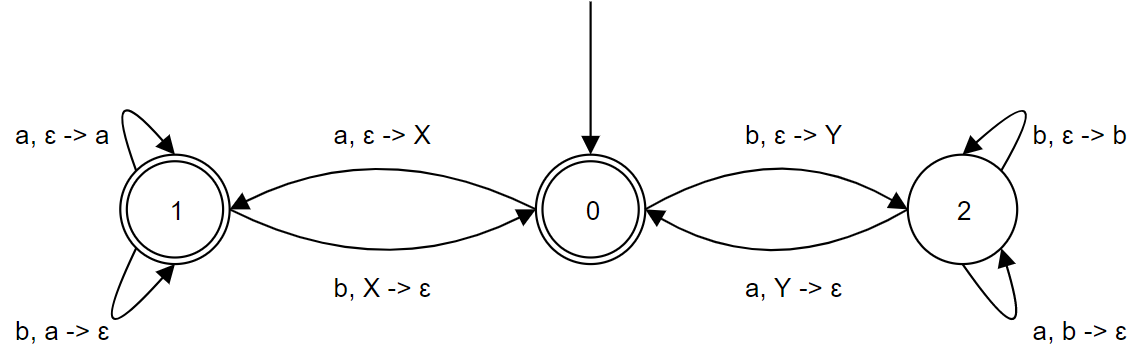
\includegraphics[width=15cm]{a2}
    When the automaton is in state '0', it means that the number of \textbf{a}s in the input string is the same as that of \textbf{b}s.\\
    When the automaton is in state '1', it means that there are more \textbf{a}s in the input string than \textbf{b}s.\\
    Symbol 'X' marks the bottom of $a$ in the stack.\\
    Symbol 'Y' marks the bottom of $b$ in the stack.
    \item
    Begin proving that every string in $L(G)$ is in $C$
        \begin{itemize}
            \item
            Base case:
            \begin{itemize}
                \item
                $\epsilon$ is in $C$ as the number of \textbf{a}s is the same as the number of \textbf{b}s.
                
                \item
                \textbf{a} is in $C$ because there are more \textbf{a}s than \textbf{b}s.
            \end{itemize}
            
            \item
            Inductive case:
            \begin{itemize}
                \item
                Consider \textbf{a} $S$ \textbf{b}. By induction hypothesis, $S$ is in $C$, so it contains at least as many \textbf{a}s as \textbf{b}s. Adding one more \textbf{a} and \textbf{b} preserves this property. So, \textbf{a} $S$ \textbf{b} is in $C$.
                
                \item
                Consider \textbf{b} $S$ \textbf{a}. By induction hypothesis, $S$ is in $C$, so it contains at least as many \textbf{a}s as \textbf{b}s. Adding one more \textbf{a} and \textbf{b} preserves this property. So, \textbf{b} $S$ \textbf{a} is in $C$.
                
                \item
                Consider $S\ S$. By induction hypothesis, $S$ is in $C$, so it contains at least as many \textbf{a}s as \textbf{b}s. Adding together the number of \textbf{a}s and \textbf{b}s in two $S$ preserves this property. So, $S\ S$ is in $C$.
            \end{itemize}
            
        \end{itemize}
    By the principle of induction, any strings in $L(G)$ are in $C$ as well.\\
    \\
    Begin proving that every string in $C$ is in $L(G)$
    \begin{itemize}
        \item
        Base case:
        \begin{itemize}
            \item
            Strings in $C$ that have length 0 = $\{\epsilon\}$ and $\epsilon$ is in $L(G)$.
            \item
            Strings in $C$ that have length 1 = $\{a\}$ and $a$ is in $L(G)$.
        \end{itemize}
        
        \item
        Inductive case:\\
        Assume that all strings in $C$ with length $n$ can be generated using $G$.\\
        Let $X$ be any string in $C$ that has length $n$. By the definition of language $C$, $X$ has at most $\frac{n}{2}$ \textbf{b}s. Using the last rule in $G$ to generate a new string, called $X'$, with length $n + 1$. $X'$ will have at least $\frac{n}{2} + 1$ \textbf{a}s and at most $\frac{n}{2}$ \textbf{b}s. So, $X'$ is in $C$.
    \end{itemize}
    
    By the principle of induction, strings with any length in $C$ are in $L(G)$ as well.\\
    \\
    Therefore, it's proved that the grammar $G$ generates $C$.
\end{enumerate}

\section*{Challenge 3}
\begin{enumerate}
    \item
    Since $R$ is regular and concatenation is a regular operation and regular languages are closed under regular operations, $R^3$ is regular.
    \item
    % $triple(R)$ is not regular. Proving using contrapositive:\\
    % Assume that $triple(R)$ is regular and it has pumping length $p$.\\
    % Consider $www \in triple(R),\ w \in R$, and $w$ has length $p$.\\
    % By pumping lemma, $www = xyz$, with $xy^iz \in triple(R)$ for all $i \geq 0$.\\
    % Since $|xy|\ \leq\ p$, $x$ contains the first part of $w$ and $y$ contains the second part. By repeating $y$ twice, the first $w$ is different from the other two, so $xyyz \notin triple(R)$.\\
    % Therefore, assumption is false and $triple(R)$ is not regular.
    $triple(R)$ is not regular. Counter-example: $R$ = \{$a^ib^j\ |\ i,\ j \geq 0$\} , which is regular. $triple(R)$ then becomes \{$a^ib^ja^ib^ja^ib^j\ |\ i,\ j \geq 0$\}.\\    
    Now, prove that $triple(R)$ is not regular by contrapositive.\\
    Assume that $triple(R)$ is regular, and has pumping length $p$.\\
    Consider $s$ = $a^pb^pa^pb^pa^pb^p$, $s \in triple(R)$.\\
    By pumping lemma, $a^pb^pa^pb^pa^pb^p$ = $xyz$, with $|xy| \leq p$ , $xy^iz \in triple(R)$ for all $i \geq 0$.\\
    $x$ and $y$ are constrained to be within the first $a^p$.\\
    Choose $i = 2$, $xyyz$ will have different number of \textbf{a}s in different segments. So, $xyyz \notin triple(R)$.\\
    Assumption is false, and $triple(R)$ is not necessarily regular, given that $R$ is regular.
    \item
    Counter-example: $R$ = \{$a^ib^jc^k\ |\ i,\ j,\ k \geq 0$\}, which is regular. $snip(R)$ then becomes \{$a^nc^n\ |\ n \geq 0$\}.\\
    Now, prove that $snip(R)$ is not regular by contrapositive:\\
    Assume that $snip(R)$ is regular and it has pumping length $p$.\\
    Consider $a^pc^p \in snip(R)$.\\
    By pumping lemma, $a^pc^p = xyz$, with $|xy| \leq p$, $xy^iz \in sinp(R)$ for all $i \geq 0$.\\
    Then, $y$ would consist entirely of \textbf{a}s.\\
    Pick $i = 2$, $xyyz \notin snip(R)$ as there are more \textbf{a}s than \textbf{c}s.\\
    Assumption is false, and $snip(R)$ is not necessarily regular given that $R$ is regular.
    % Consider $ab \in snip(R)$, with length of sub-string $a$ and sub-string $b$ being equal to $p$.\\
    % By pumping lemma, $ab = xyz$, with $xy^iz \in snip(R)$ for all $i \geq 0$.\\
    % According to the definition of $snip(R)$, all strings in it has even length.\\
    % The length of $xy^iz$ is not going be even for all $i > 0$, so $x^iz \notin triple(R)$ for all $i > 0$\\
    % Therefore, assumption is false, and $sinp(R)$ is not regular.
\end{enumerate}

\end{document}
